\documentclass[11pt, a4j]{jreport}

\usepackage{comment}
\usepackage{float}
\usepackage{color}
\usepackage{multicol}
\usepackage[dvipdfmx]{pict2e}
\usepackage{wrapfig}
\usepackage{graphicx}
\usepackage{bm}
\usepackage{url}
\usepackage{underscore}
\usepackage{colortbl}
\usepackage{tabularx}
\usepackage{fancyhdr}
\usepackage{ulem}
\usepackage{amsmath, amssymb, amsfonts}
\usepackage{algorithmic}
\usepackage{textcomp}
\usepackage{xcolor}
\usepackage[ipaex]{pxchfon}
\usepackage{otf}
\usepackage[round]{natbib}
\bibliographystyle{plainnat}

\usepackage[top=30truemm, bottom=30truemm, left=25truemm, right=25truemm]{
    geometry
}

% 図や表のナンバリングを章に依存せず、通し番号にする設定
\renewcommand{\thefigure}{\arabic{figure}}
\renewcommand{\thetable}{\arabic{table}}

\begin{document}
    \thispagestyle{empty}
    \begin{center}
        \vspace{20mm}
        {\Large\noindent 2024年度 卒業論文}\\
        \vspace{40mm}
        {\huge\noindent\textbf{SNSにおける世論形成と紛争に関する\\
        Reddit投稿分析}}\\
        \medskip
        {\huge\noindent\textbf{ーイスラエルによるレバノン侵攻を例にー}}\\
        \vspace{\baselineskip}
        \vspace{40mm}
    
        {\Large\noindent グローバル地域文化学部 アジア・太平洋コース \\ 
        \vspace{\baselineskip} 学生ID: 1122192047 氏名: 種村尚大\\
        \vspace{\baselineskip} 指導教員: \CID{8443}田智子 }
        \vspace{40mm}
    \end{center}

    \thispagestyle{empty}
    \clearpage

    %=====================================================================================

    \begin{center}
        {\Large 2024年度 卒業論文} \\[5mm]
        {\Large \textbf{SNSにおける世論形成と紛争に関する\\
        Reddit投稿分析\\
        ーイスラエルによるレバノン侵攻を例にー}} \\[15mm]
    \end{center}
    
    % 学生情報
    \noindent
    グローバル地域文化学部 アジア・太平洋コース \\
    学生ID : 1122192047 氏名: 種村尚大 \\
    指導教員 : \CID{8443}田智子 \\[15mm]
    
    % 論文要旨
    \noindent
    {\Large \textbf{論文要旨}} \\[5mm]
    \quad 本研究は、2024年10月1日に発生したイスラエルによるレバノン侵攻を契機に、SNS上の議論がどのように形成され、進展していくのかを探ることを目的とした。具体的には、Redditの投稿データを用い、投稿数の変動、感情的傾向、トピックの変遷を分析することで、SNSが紛争に与える影響を多角的に検討した。\\
    \quad 研究の結果、投稿数が急増する一方で、センチメントスコアがポジティブにシフトする現象が確認された。また、動的トピックモデリングを用いて、議論が「紛争と軍事行動」から「規則や投稿削除」といったメタ的テーマへと移行する過程を明らかにした。この分析を通じて、SNSが国際紛争におけるデジタル公共圏として機能する一方で、議論の構造や偏りに関する課題があることも示された。本研究の知見は、SNSを活用した情報戦略や政策設計における実践的な示唆を提供するものである。 \\[20mm]
    
    % キーワード
    \noindent
    {\Large \textbf{キーワード}} \\[5mm]
    SNS, Reddit, 国際紛争, 世論形成, データ分析
    %=====================================================================================

    % 目次の表示
    {\makeatletter
    \let\ps@jpl@in\ps@empty
    \makeatother
    \pagestyle{empty}
    \tableofcontents
    \clearpage}
    %=====================================================================================
    \pagestyle{plain}
    \lhead{\rightmark}
    \renewcommand{\chaptermark}[1]{\markboth{第\ \normalfont\thechapter\ 章~~#1}{}}
    %=====================================================================================

    \chapter{はじめに} %章
    \setcounter{page}{1} % 第一章の開始ページからページ番号を振る

    \section{研究背景}

    21世紀における紛争の様相は、従来の軍事的な衝突に加え、情報空間における戦いの重要性が増している。特に、ソーシャルネットワーキングサービス(SNS)は、紛争に関する情報発信や議論の場として機能し、世論形成に強い影響を与えている。これらのプラットフォームは、リアルタイムでの情報共有、国際的な議論の可視化、多様な声の拡散を可能にしている。

    中でもRedditは、特異な構造と利用者特性を持つSNSとして注目されている。Redditは2005年に設立され、2024年時点で日毎のアクティブユーザー数が約9720万人に達している\citep{reddit2024third-quater-results}。その利用者層は主に北米とヨーロッパに集中しており\citep{statista2024reddit-country}、ユーザーの約44\%が18~29歳と比較的若い世代に偏っている\citep{statista2024reddit-age}。また、性別比率では男性が約60\%を占めるが、女性ユーザーも年々増加傾向にある\citep{statista2024reddit-gender}。さらに、Redditのユーザーは教育水準が高く、大学卒業者が多いことも特徴の一つである\citep{pew2024reddit-educated}。

    このプラットフォームの最大の特徴は、匿名性と分散型のコミュニティ構造にある。Redditは、サブレディットと呼ばれる膨大な数の専門的なコミュニティで構成されており、それぞれが特定のトピックや興味に基づいて議論を展開する。投稿やコメントは、ユーザーからの評価(アップボートまたはダウンボート)によってランキングされるため、コミュニティ全体の関心や優先順位が自然に反映される仕組みが採用されている。この構造は、特定の話題について多様な視点を集約し、リアルタイムで議論を活発化させる基盤を提供している。

    2024年10月1日にイスラエルが実施したレバノン侵攻は、国際社会における注目を集め、地域的な緊張を一層高める結果となった。この侵攻は、南レバノンを拠点とする武装組織ヒズボラによる攻撃への報復として行われたが、同時に人道危機を引き起こし、多くの民間人が犠牲となった。国連や人権団体は、即時停戦を呼びかける一方で、戦闘行為によるインフラの破壊と大規模な避難民の発生について深い懸念を表明した。

    このような状況の中、SNS上の議論は急激に活発化し、Redditでも紛争関連の投稿やコメントが急増した。特に、r/worldnews, r/politics, r/MiddleEastなどのサブレディットでは、侵攻に関する情報や意見交換が爆発的に広がり、国際社会の反応や一般ユーザーの感情がリアルタイムで可視化された。これらのプラットフォームは、紛争に関連する多様な視点を集約するだけでなく、特定の意見やナラティブがどのように形成され拡散するかを観察する上で極めて重要な役割を果たした。

    本研究では、このReddit上で観察される投稿数や感情の変化、議論のトピックの移り変わりを分析し、現代の紛争がデジタル空間でどのように議論されるのかを探る。

    \section{研究目的}
    本研究の目的は、2024年10月1日に発生したイスラエルによるレバノン侵攻がReddit上の議論やユーザーの反応にどのような影響を与えたかを明らかにすることである。具体的には、投稿数の変動、感情的傾向の変化、トピックの変遷という三つの観点からこの影響を分析する。紛争の発生が投稿数にどのような変化をもたらしたのかを評価することで、議論の活性化や関心の高まりを測定する。また、感情分析を用いて紛争に対するユーザーの反応が時間とともにどのように変化したのかを明らかにする。そして、動的トピックモデリング(DTM)を活用することで、議論が紛争直後の急性期からその後の段階に至るまでどのように展開したのかを時系列で追跡する。
    
    さらに、本研究はRedditという匿名性と分散型構造を持つSNSプラットフォームの特性に着目し、この特性が国際紛争に関する議論に与える影響を詳細に分析することを目指す。投稿数や感情スコアの分析に加え、トピックモデリングを活用することで、議論がどのようにテーマを移行させていくのかを具体的に示す。また、サブサンプリングや差分の差分(DID)分析を用いることで、紛争発生という介入が議論の量的および質的側面にどのような因果的影響を与えるのかを評価する。これらの分析を通じて、SNSが国際紛争に与える影響を総合的に理解するためのデータ駆動型の知見を提供する。
    
    本研究は、Redditという特異なプラットフォームにおける議論のダイナミクスを解明することで、デジタル時代の国際紛争におけるSNSの役割を理解するための新たな知見を提供することを目指している。また、この研究は、政策立案者や国際機関がデジタル空間を活用する際の参考となり得る重要な示唆を含むものである。

    \section{本論文の仮説}
    本研究では、以下の三つの仮説を検証する。まず、イスラエルによるレバノン侵攻が紛争関連サブレディットにおける投稿数を急増させる一方で、対照群では投稿数の変化が限定的であると考えられる。次に、紛争直後に投稿内容はネガティブかつ感情的な傾向を示し、センチメントスコアが低下すると仮定する。最後に、紛争に関する議論は、発生直後には戦闘や人道危機に集中し、時間の経過とともに国際支援や解決策の模索へと焦点が移ると想定する。
    
    \section{本論文の構成}
    本論文は以下の構成をとる。第2章では、SNSにおける世論形成と国際紛争に関する先行研究をレビューし、Redditの特性について議論する。第3章では、データ収集および分析手法を詳述し、投稿数、センチメントスコア、トピックの変化を調査するための具体的な方法論を提示する。第4章では、分析結果を提示し、紛争がReddit上の議論に与える影響を示す。第5章では、結果を解釈し、SNSが国際紛争における世論形成や情報拡散に果たす役割について考察する。第6章では、本研究の結論をまとめ、今後の課題と研究の展望を示す。

    \chapter{SNSにおける世論形成と国際紛争に関する先行研究}

    \section{SNSと世論形成}
    ソーシャルネットワーキングサービス(SNS)は、21世紀において世論形成の重要なツールとなり、従来のマスメディアを補完する役割を果たしている。特に、情報が瞬時に広範囲に拡散され、多様な意見が可視化される点で、SNSは「集団行動を促進するツール」として位置づけられている\citep{shrinky2011}。例えば、2010年代の「アラブの春」では、TwitterやFacebookを通じて市民がプロテストの呼びかけや情報共有を行い、社会運動の大規模化を支えたことが報告されている\citep{howard-hussain2013}。このように、SNSは社会的・政治的な動員における迅速性と規模の拡大に寄与している。

    一方で、SNSにおける情報流通には限界も指摘されている。\citet{ulen2001democracy}やPariser\citet{pariser2011filter}は、エコーチェンバー現象やフィルターバブルが、ユーザーを特定の情報に偏らせるリスクを指摘している。たとえば、Facebookのアルゴリズムによるフィードの最適化が、政治的分断を助長する可能性があることが示されている。これらの現象は、SNSが多様な意見の交換を促進する一方で、逆に対話の閉鎖性を生む可能性があることを示唆している。

    さらに、SNSが選挙や緊急事態において果たす役割も注目されている。たとえば、2016年のアメリカ大統領選挙では、Twitterを通じての情報戦が候補者のイメージ形成に影響を与えたことが明らかにされている\citep{allcott-gentzkow2017}。このように、SNSの利用は単なる情報共有を超え、世論形成における戦略的な要素としても機能している。

    \section{国際紛争におけるSNSの役割}
    SNSは国際紛争において、単なる情報共有の場を超え、プロパガンダや情報操作の場としても機能している。\citet{howard-hussain2013}は、アラブの春におけるSNSの役割について、情報の共有と抗議活動の組織化を促進する手段としての重要性を指摘している。また、\citet{zeitzoff2017}の研究では、イスラエルとハマスの紛争におけるTwitterの使用が、紛争当事者のソフトパワー的な戦略に寄与していることが示されている。たとえば、戦闘の進行状況をリアルタイムで伝えることで、国際的な支持を獲得する動きが観察されている。

    さらに、SNSは国際的な議論を加速させるツールとしても機能している。イスラエルとパレスチナの紛争では、世界中のユーザーがSNSを通じて意見を発信し、国際世論が紛争当事者への外交的プレッシャーとして作用するケースが見られる。これにより、SNSは紛争解決や国際支援のプロセスに間接的な影響を及ぼしている。

    \citet{bennett2013logic}は、SNSが「ネットワーク化された個人的行動」を促進し、従来の組織化された抗議活動よりも分散的で迅速な動員を可能にすると述べている。この視点は、SNSが国際紛争の文脈において、情報共有だけでなく、個人の行動を直接的に動員する力を持つことを示唆している。

    \section{Redditの特異性}
    Redditは他のSNSと比較して匿名性が高く、ユーザーが特定のトピックに関心を持つコミュニティ(サブレディット)に参加することで、多様な意見交換が可能となるプラットフォームである。\citet{massanari2015participatory}は、Redditの匿名性と分散型構造が、多様な視点を反映した議論を促進すると指摘している。また、「アップボート」「ダウンボート」の評価システムは、特定の意見が可視化される一方で、少数派の意見も一定の支持を得て拡散される可能性を持つ。

    特に、国際紛争に関する議論では、サブレディットごとに異なる視点が展開されることが多い。たとえば、「r/worldnews」ではグローバルな視点からの議論が行われる一方、「r/Israel」や「r/palestine」では地域特有の視点が強調される。\citet{gaffney2018caveat}の研究によれば、Redditのコメントシステムは階層的な議論構造を生み出し、紛争の複雑な側面に関する多層的な議論を可能にしている。この特徴は、他のSNSでは観察されにくいReddit特有の性質といえる。

    さらに、Redditのサブレディットは、特定のトピックや価値観を共有するユーザーが集まることで結束を強化する特徴を持つ。\citet{massanari2015participatory}は、Redditの匿名性と分散型構造が、多様な意見を反映しつつも、特定のコミュニティにおける共有された価値観や視点の強化につながると指摘している。\citet{gaffney2018caveat}も、Redditのコミュニティ構造が特定の議論を深める場として機能する一方で、ユーザー間の結束を促進する仕組みを提供していることを示している。

    \section{先行研究との関係}
    これまでの先行研究は、SNSが国際紛争や政治的動員に与える影響について、SNS全般の役割や、主にTwitterやFacebookといったプラットフォームの影響を分析してきた。たとえば、\citet{shrinky2011}や\citet{howard-hussain2013}は、SNSがプロテスタントや社会運動の組織化を支援し、情報拡散を迅速化するツールとしての役割を強調している。また、\citet{zeitzoff2017}はTwitterを用いて、紛争当事者が戦略的なコミュニケーションを通じて国際的な支持を獲得する手段としてSNSを活用していることを示している。しかし、これらの研究は、特定のプラットフォームの独自性や、ユーザー間の議論ダイナミクスの詳細には踏み込んでおらず、SNSが個々のユーザーやコミュニティの世論形成にどのように作用するかについては限定的である。

    本研究は、これらの先行研究に対して以下の3つの点の視点を示すという、学術的意義を有する。

    \subsection{Redditという未開拓プラットフォームへの着目}
    既存の研究の多くがTwitterやFacebookといった既成のSNSに焦点を当てている中で、本研究はRedditという匿名性が高く、分散型構造を持つプラットフォームを対象としている。Redditの特異性は、サブレディットというコミュニティ構造と、ユーザーがコンテンツを評価する投票システムにある。この特徴は、議論が多様な視点を含む形で展開される可能性を高める一方で、議論の偏りや極化を生むリスクも持つ。\citet{massanari2015participatory}が示すように、Redditの評価システムは、少数意見や論争的な意見の可視性を保証する仕組みとして機能しており、これが世論形成に与える影響は他のSNSとは一線を画す。

    特に、本研究は、イスラエル・レバノン紛争という具体的な国際事件を題材に、Reddit上での議論のダイナミクスを分析することで、このプラットフォームが国際紛争に関連する世論形成や情報拡散に与える独自の影響を明らかにする。

    \subsection{データ駆動型アプローチの統合}
    従来のSNS研究では、投稿数の変化や感情分析を用いた傾向の把握が主流であった。本研究ではこれらの手法に加え、動的トピックモデリング(DTM)を用いた議論のテーマの変遷分析を組み合わせることで、議論の量的変化だけでなく、その質的側面を時系列的に明らかにすることを試みる。

    具体的には、投稿数の急増やセンチメントスコアの変化を検出するだけでなく、DTMを活用して、議論が「戦闘」「人道危機」「国際支援」などのトピックにどのように分布し、時間の経過とともにどのように移行していくかを分析する。この手法により、投稿者の関心がどの時点で特定のテーマに集中し、その後どのように新たなトピックへと推移していくかを詳細に把握することが可能となる。

    特に、紛争直後における投稿数や感情の急激な変化が、どのようなテーマと関連しているのかを検討することで、SNS上の議論形成のダイナミクスをより深く理解するための基盤を提供する。本研究のように量的データ(投稿数やセンチメントスコア)と、トピックという質的側面を統合的に分析するアプローチは、SNS研究における新たな視点を提供するとともに、議論の全体像をより包括的に捉えることに寄与する。

    \subsection{国際紛争とオンライン世論の関係性への新たな知見}
    既存研究では、SNSが国際紛争において果たす役割が、情報拡散やプロテスタントの動員といった「直接的な効果」に焦点を当てることが多かった。一方で、本研究は、Reddit上の議論が紛争当事者への国際的な支持や批判を形成するだけでなく、SNS利用者同士の議論の焦点やトーンがどのように変化し、SNS全体の議論空間に影響を与えるかを検証する。具体的には、サブレディット間での視点の違いや、特定のテーマに対する議論の偏りが、紛争の認識や世論形成に与える影響を多角的に分析する。

    また、Redditが持つ匿名性や分散型構造の特性が、議論の質や偏りにどのように影響するかについても考察することで、従来のSNS研究では見落とされてきた議論の「質的側面」に光を当てる。この点で、本研究は単なる議論の量的変化にとどまらず、その内容や構造の変化を深く掘り下げる。

    \subsection{SNS研究への学術的貢献と実践的意義}
    本研究は、Redditという未開拓のプラットフォームを対象とすることで、SNS研究に新たな学術的貢献を提供する。また、紛争や国際問題における世論形成のプロセスを明らかにすることは、政策立案者や国際機関にとって、SNSを活用した情報戦略の策定やデジタルディプロマシーの構築に向けた実践的な示唆を提供する。

    \chapter{データ収集・分析手法}
    本章では、Redditにおける投稿データを対象としたデータ収集および分析手法について詳述する。本研究では、信頼性と精度を確保しつつ、大規模な投稿データを効率的に取得するために適切なデータ収集アプローチを採用した。さらに、収集したデータを用いて、投稿数の変化、センチメントスコアの推移、および議論のトピックの変遷を分析するための方法論を提示する。これにより、データ駆動型の手法が本研究の目的を達成する上でなぜ有効であるかを論じる。

    \section{データ収集の方法}
    \subsection{PRAWを用いたデータ収集}
    Redditのデータ収集には、PRAW (Python Reddit API Wrapper) を主に使用し、大規模かつ効率的なデータ取得を実現した。

    収集対象期間は、イスラエルによるレバノン侵攻(2024年10月1日)の影響を分析するため、2024年7月26日から2024年10月26日までの約3ヶ月間とした。この期間設定により、紛争勃発前の基準値、直後の急激な反応、そしてその後の議論の推移までを包括的にカバーできる。

    対象となるサブレディットは、イスラエル・パレスチナ問題に関連する議論が活発な「r/Israel」「r/Palestine」「r/IsraelPalestine」の3つに加え、対照群として、紛争と無関係な一般的なサブレディット「r/ps4homebrew」「r/Exercise」「r/voyageons」も収集した。これにより、紛争関連サブレディットにおける変化を対照的に比較する枠組みを構築した。

    データとしては各サブレディットにおけるsubmissionとそれに付随してコメントも取得対象とした。

    \section{投稿数の変化と差分の差分(DID)分析}
    投稿数の変化を分析するため、Pythonのmatplotlibおよびpandasライブラリを用いて時系列データを可視化した。データは1日単位で集計し、紛争勃発日(2024年10月1日)を基準として、紛争前後での投稿数の変動を比較した。

    さらに、紛争の影響を定量的に評価するため、差分の差分(Difference-in-Differences, DID)分析を実施した。DIDは観察データに基づき介入(今回の場合は紛争勃発)が結果に与える因果的な影響を推定する手法であり、紛争関連サブレディットと対照群サブレディットの間での投稿数の変化を比較することで、介入の純粋な効果を明らかにすることが可能である。

    \subsection{サブサンプリングによるデータ調整}
    分析対象となるデータでは、処置群(紛争関連サブレディット)の投稿数が対照群(非紛争関連サブレディット)と比較して大幅に多いことが確認された。このデータの不均衡は、DID分析における結果の偏りや推定値の信頼性低下を招く可能性がある。そのため、対照群サブレディットの日次投稿数の平均を基準として、処置群からランダムに同数の投稿を抽出するサブサンプリングを実施した。さらに、このサブサンプリングは分析結果の安定性を確保するために複数回(100回)繰り返し行われ、その平均値が算出された。最後に、サブサンプリングによって調整されたデータを用いてDIDモデルを適用した。

    このプロセスにより、処置群と対照群のデータ数の差を緩和し、DID分析における比較の公平性と信頼性を向上させた。この処理は後ほど説明する「感情分析とVADERスコアの時系列変化」でも同様に実施されている。

    \subsection{DIDを用いる必要性}
    DID分析を採用した理由は三つある。まず、介入の因果的影響を識別するためである。紛争勃発による投稿数の変化を単に観察するだけでは、紛争以外の要因、例えば季節的な投稿数の変動や一般的なトレンドなどが結果に影響を与えている可能性を排除することはできない。DIDを用いることで、紛争関連サブレディット(処置群)と、紛争と無関係なサブレディット(対照群)を比較し、これらの外的要因を統制しつつ紛争の影響そのものを識別することが可能になる。
    
    次に、差分の差分に基づく純粋な影響推定を行える点である。DIDでは、まず介入前後で処置群(紛争関連サブレディット)の投稿数変化を計算し、次に介入前後で対照群(非紛争関連サブレディット)の投稿数変化を計算する。そして、処置群と対照群の変化量を比較(差分の差分)することで、介入の純粋な影響を推定する。これにより、紛争がなかった場合の投稿数変化を対照群の変化を基に推定し、それをコントロールすることで、紛争の影響を明確にすることができる。
    
    最後に、観察データに基づく実践的な有用性が挙げられる。DIDは、ランダム化実験が実施できない場合においても因果推論を行うために広く用いられる手法である。今回のケースでは、紛争が自然発生的な事象であり、介入のタイミングを研究者が制御できないため、DIDは適切な分析手法といえる。

    \subsection{DIDモデルの仕様}
    DID分析では、以下の回帰式を使用した。

    \begin{equation}
        Y_{it} = \beta_{0} + \beta_{1}*Treatment_{i} + \beta_{2}*Post_{t} + \beta_{3}*(Treatment_{i} * Post_{t}) + \epsilon_{it}
    \end{equation}

    この回帰式において、各パラメーターは以下のような意味を持つ。
    \begin{itemize}
        \item $Y_{it}$:日次投稿数(サブレディット$i$の時点$t$における投稿数)
        \item $Treatment_{i}$:紛争関連サブレディットであるか否か(1=処置群、0=対照群)
        \item $Post_{t}$:紛争勃発後の期間であるか否か(1=紛争後、0=紛争前)
        \item $(Treatment_{i} * Post_{t})$:処置群で紛争後の期間を示す相互作用項
        \item $\beta_{3}$:紛争の影響を表す推定値
    \end{itemize}

    \subsection{DIDの意義と期待される結果}
    DID分析の結果、$\beta_{3}$の推定値が正で有意であれば、紛争が紛争関連サブレディットの投稿数を有意に増加させたことを意味する。これにより、紛争がReddit上の議論活性化に与える直接的な影響を実証的に評価することが可能となる。

    また、対照群サブレディットを使用することで、紛争以外の要因(例:一般的な投稿数の増減、システム的な変化など)が分析結果に与える影響を排除し、結果の信頼性を高める。

    \section{感情分析とVADERスコアの時系列変化}

    \subsection{VADERの仕組みとその意義}
    感情分析には、VADER(Valence Aware Dictionary and sEntiment Reasoner)を使用した。VADERは、ソーシャルメディアのような非構造化テキストに適した辞書ベースの感情分析ツールであり、短文、スラング、絵文字、強調表現(例:「!!!」「VERY」)などを含む多様な文脈を効果的に処理できるよう設計されている。

    VADERのアルゴリズムは、辞書に基づくアプローチを採用しており、単語やフレーズに事前に割り当てられたセンチメントスコア(ポジティブ、ネガティブ、中立)を元に、文章全体のセンチメントスコアを計算する。この辞書は、人間の評価者がラベル付けを行ったデータセットに基づいて構築されており、特にソーシャルメディアやニュースの文脈での利用を想定して作成されている。

    VADERが広く利用される理由は三つある。第一に、ソーシャルメディア特有のスラングや絵文字、文脈的な意味を考慮できる点が挙げられる。これにより、従来の感情分析手法が見落としがちなソーシャルメディア特有の言語表現にも対応可能である。第二に、ポジティブ、ネガティブ、ニュートラルといったスコアに加えて、総合的な「コンパウンドスコア」を提供することで、文全体の感情を包括的に評価できる点が特長である。最後に、Pythonライブラリに統合されているため、高速かつ簡便な処理が可能であり、実用性が高い。このように、VADERはソーシャルメディアにおける感情分析において非常に有用なツールとなっている。

    今回の分析においてVADERを使用する意義は、Reddit投稿が一般的な形式的文章とは異なり、インフォーマルで感情的な表現が多く含まれることにある。VADERは、これらの特徴を考慮した感情分析が可能であり、紛争前後における投稿者の感情的な反応を効果的に捉えるツールとして最適である。

    \subsection{紛争前後の感情変化の分析とDIDの必要性}
    VADERスコア(ポジティブ、ネガティブ、中立)を日次で集計し、センチメントスコアの変化を紛争前後で比較した。また、センチメントスコアの変化をより定量的に評価するため、DID(差分の差分)分析を適用した。

    DID分析を採用した理由は二つある。第一に、因果関係を識別するためである。紛争関連サブレディット内のスコアを単に比較するだけでは、紛争の影響以外の要因、例えば一般的な季節変動やイベントによるスコア変動が結果に影響を及ぼす可能性がある。この点でDID分析は、対照群(非紛争関連サブレディット)と比較することで、紛争そのものがセンチメントスコアに与えた影響を識別するための適切な方法となる。
    
    第二に、純粋な介入効果を抽出するためである。DID分析は、紛争前後での処置群(紛争関連サブレディット)のセンチメントスコア変化と、対照群の変化を比較することで、紛争がセンチメントスコアに与えた純粋な影響を明らかにすることができる。このように、DID分析は本研究の目的において重要な役割を果たす手法である。

    DID分析では、以下の回帰式を使用した。
    \begin{equation}
        Sentiment_{it} = \beta_{0} + \beta_{1}*Treatment_{i} + \beta_{2}*Post_{t} + \beta_{3}*(Treatment_{i} * Post_{t}) + \epsilon_{it}
    \end{equation}

    この回帰式において、各パラメーターは以下のような意味を持つ。
    \begin{itemize}
        \item $Sentiment_{it}$:日次VADERセンチメントスコア(ポジティブ、ネガティブ、またはコンパウンドスコア)
        \item $Treatment_{i}$:紛争関連サブレディットであるか否か(1=処置群、0=対照群)
        \item $Post_{t}$:紛争後の期間であるか否か(1=紛争後、0=紛争前)
        \item $\beta_{3}$:紛争がセンチメントスコアに与える影響を表す推定値
    \end{itemize}

    \subsection{分析結果の意義}
    DID分析により、紛争勃発後、紛争関連サブレディットでセンチメントスコアがネガティブにシフトし、対照群では顕著な変化が見られないことを示す。これにより、紛争がオンライン議論に与える感情的影響を明確にし、Reddit上の議論のダイナミクスを深く理解するための基盤を提供する。

    \section{トピックモデリングによるテーマ分析}
    投稿内容のテーマを分析するため、LDA(潜在ディリクレ配分)ではなく、動的トピックモデリング(Dynamic Topic Modeling, DTM)を採用した。この手法は、議論のトピックが時間とともにどのように変遷するかを詳細に分析することを可能にする。

    DTMの実施手順は次の通りである。まず、テキストの前処理を行い、トークン化、ストップワードの除去、ステミングを実施する。その後、文書-単語行列を作成し、時系列データに基づいてDTMモデルを構築する。このモデルを用いて、各週ごとの主要トピックとその割合を推定し、最後にトピックごとの時間的推移を可視化する。これらの手順を通じて、DTMの分析が進められる。

    \section{分析手法の有効性}
    本研究で採用した分析手法は、Redditにおけるユーザーの反応を多角的に捉えることを目的としている。特に投稿数や感情の変化を定量的に分析する手法と、投稿内容の詳細な特徴を捉える方法を組み合わせることで、データ駆動型の分析と実証的な議論を可能にしている。それぞれの手法の有効性について以下に論じる。

    \subsection{投稿数およびセンチメントスコアの変化に関する定量的分析の有効性}
    定量的分析は、大規模データセットの全体的な傾向を把握し、外部要因(例: 紛争勃発)がReddit上の議論に与える影響を評価する上で有効である。本研究では、投稿数とセンチメントスコアの変化を時系列で分析し、さらにDID(差分の差分)分析を用いて因果関係を特定する。

    DID分析は、自然実験的状況下での因果推論を行うのに適した手法であり、紛争関連サブレディット(処置群)と非関連サブレディット(対照群)間の変化を比較することで、紛争が議論活性化や感情表現に与える影響を厳密に評価できる。この手法にサブサンプリングを組み合わせることで、処置群と対照群のデータ数の不均衡を調整し、分析結果の公平性と信頼性を高めることができる。

    また、センチメントスコアにはVADER(Valence Aware Dictionary and sEntiment Reasoner)を使用した。VADERはSNSデータに特化して設計されており、スラング、絵文字、文脈依存の表現を効果的に処理する機能を持つ。これにより、投稿のポジティブ、ネガティブ、中立的な感情の傾向を時間軸に沿って分析することが可能となり、重要なイベントに対するユーザーの感情的反応を定量的に評価することができる。

    \subsection{投稿内容の分析に関するアプローチの有効性}
    本研究では、感情分析を補完する形で、投稿内容に含まれる具体的なトピックやテーマの変遷を捉えるため、動的トピックモデリング(DTM)を採用した。この手法は、投稿データをトピックに分解し、時間の経過とともに議論の焦点がどのように移行するかを詳細に明らかにする。

    DTMの利点は、テーマの変化を定量化しつつ、データ駆動型の方法で隠れた構造を発見できる点にある。これにより、紛争に関連する議論が「戦闘」「人道的危機」「国際的対応」といったテーマから、議論のルールや行動規範のようなメタレベルの議論へと移行する過程を捉えることができる。

    \section{分析手法の限界}
    本研究で採用した分析手法にはいくつかの限界が存在する。
    
    \subsection{データ収集の限界}
    Reddit上の投稿が全て人間によるものではなく、一部にはボットやスパム投稿が含まれる可能性がある。この問題に対処するためには、投稿パターンやユーザー履歴を基にボットを検出・除外するアルゴリズムの実装が必要であるかもしれない。また、今回の分析ではRedditの特定のサブレディットに焦点を当てたため、他のSNSや他のサブレディットのデータを取り入れることで、より包括的な結果が得られる可能性がある。
    
    さらに、データ収集においては、Reddit APIの仕様や制限に依存しているため、潜在的なデータ欠損や取得漏れが発生する可能性がある。特に、削除された投稿やコメント、特定のユーザーによる非公開設定など、分析対象から除外されるデータが存在することが問題となる。また、サブレディットの選定には一定の偏りが含まれる可能性があり、議論の内容や性質が投稿者の意見や視点に大きく左右されるため、結果の解釈には注意が必要である。
    
    \subsection{感情分析の限界}
    感情分析に使用したVADERはSNSデータに適している一方で、文脈や文化的な違いに起因するニュアンスの違いを完全には捉えられない可能性がある。特に、皮肉や隠喩、暗喩の多用がセンチメントスコアの精度に影響を与える。この問題に対処するため、一部のデータについて人間のコーディングによる検証を行い、機械的な分析結果を補完する必要がある。
    
    また、VADERの辞書ベースのアルゴリズムでは、高度な文脈依存の表現を完全に捉えることは難しい。例えば、同じ単語やフレーズが異なる文脈で異なる意味を持つ場合、その違いを適切に評価できない可能性がある。これにより、特定の投稿における感情的なニュアンスが十分に反映されない場合がある。
    
    \subsection{DID分析の限界}
    DID分析においては、平行トレンド仮定が完全に満たされていない場合、推定結果に歪みが生じる可能性がある。特に、紛争関連サブレディットと非関連サブレディットの間での投稿数の変動要因が本質的に異なる場合、この仮定が崩れることが懸念される。さらに、DIDモデルの適用に際して処置群と対照群のデータ数に不均衡があることも分析結果に影響を与える可能性がある。

    \section{まとめ}
    本章では、Redditにおける投稿データを用いたデータ収集および分析手法について詳細に論じた。本研究では、Pushshift APIを用いた効率的なデータ収集手法を採用し、投稿数の変化、センチメントスコアの推移、議論のトピックの変遷を明らかにするための多様な分析手法を組み合わせたアプローチを採用している。

    特に、投稿数の時系列分析、VADERを用いた感情分析、動的トピックモデリング(DTM)によるテーマの変遷分析などを組み合わせることで、単なる投稿数の増減だけでなく、議論の焦点や感情的な傾向、そしてこれらが時間の経過とともにどのように推移するかを総合的に把握することが可能となる。これらの手法は、紛争や政治的イベントに対するユーザーの反応をより深く理解するための有効な手段であるといえる。

    また、本研究のデータ収集や分析において直面する限界と、それに対する具体的な対策についても議論した。例えば、処置群と対照群間のデータ数の不均衡に対応するためのサブサンプリングや、感情分析における文化的・文脈的な違いを考慮するための補完的な手法の必要性を指摘した。

    次章では、これらの手法に基づいて得られた実際の分析結果を提示する。具体的には、ハマス・イスラエル紛争に関連するReddit上での議論がどのように変化し、どのような特徴を持つのかを詳細に検討する。この分析結果は、SNSが国際紛争における世論形成に与える影響を理解するための重要な知見を提供するとともに、デジタル空間における議論の動態を捉える新たな視点を示すものである。

    \chapter{データ分析結果}
    本章では、Redditから収集した投稿データを基にしたデータ分析結果を示す。対象サブレディット「r/Palestine」「r/Israel」「r/IsraelPalestine」の投稿数およびセンチメントスコアの変化、トピックモデリングの結果を通じて、SNS上における世論の動向とその変化を明らかにする。

    \section{投稿数の変化}
    10月1日のイスラエルによるレバノン侵攻を境に、投稿数にどのような変化が生じたかをOLS回帰分析により検証した。その結果、侵攻後の投稿数において統計的に有意な増加が観察された。特に、群間の交互作用効果(\textit{interaction})が有意であり($p = 0.032$)、侵攻後の特定サブレディットにおける投稿数の増加が確認された。

    表\ref{tab:ols_counts_results}は回帰結果を示している。

    \begin{table}[H]
        \centering
        \resizebox{\textwidth}{!}{
        \begin{tabular}{|c|c|c|c|c|c|c|}
            \hline
            変数 & 回帰係数(coef) & 標準誤差(std err) & t値(t) & $P>|t|$ & 95\%信頼区間(下限) & 95\%信頼区間(上限) \\
            \hline
            定数項(Intercept) & 143.9231 & 11.681 & 12.321 & 0.000 & 120.900 & 166.946 \\
            群(group) & -16.4923 & 16.520 & -0.998 & 0.319 & -49.052 & 16.067 \\
            侵攻後(post\_treatment) & -21.4022 & 17.923 & -1.194 & 0.234 & -56.727 & 13.923 \\
            交互作用(interaction) & 55.6691 & 25.767 & 2.161 & 0.032 & 4.884 & 106.454 \\
            \hline
        \end{tabular}
        }
        \caption{投稿数の変化に関するOLS回帰結果}
        \label{tab:ols_counts_results}
    \end{table}

    主な観測結果としては以下の通りである。定数項(\textit{Intercept})については、基本的な投稿数の平均が約143.92件であり、この結果は統計的に有意であった($p < 0.001$)。群の効果(\textit{group})に関しては、群間の差異は統計的に有意ではないと示された($p = 0.319$)。次に、侵攻後の効果(\textit{post\_treatment}))では、全体的な投稿数の減少傾向が観察されたものの、この結果は有意ではなかった($p = 0.234$)。一方で、交互作用効果(\textit{interaction})については、侵攻後の特定群において投稿数が約55.67件増加しており、この効果は統計的に有意であることが確認された($p = 0.032$)。

    また、図\ref{fig:submissions_comments_trends}は日毎の投稿数の推移を示している。
    \begin{figure}[H]
        \centering
        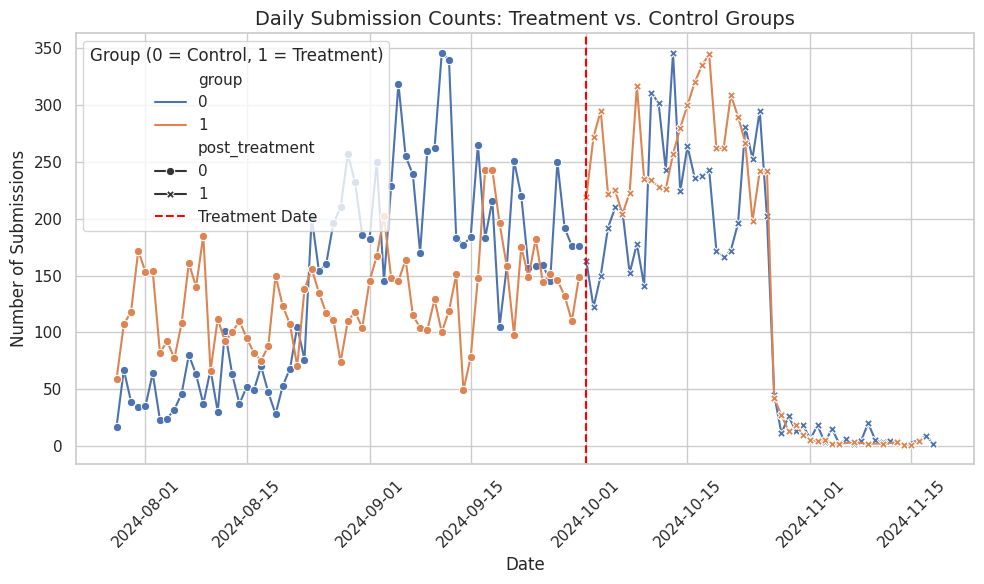
\includegraphics[width=0.8\textwidth]{submission_count_plot.png}
        \caption{日ごとの投稿数の推移(2024年7月~11月)}
        \label{fig:submissions_comments_trends}
    \end{figure}

    以上の結果は、侵攻後に特定のサブレディットにおいて投稿数が有意に増加したことを示している。この変化は表\ref{tab:ols_counts_results}における交互作用効果によって裏付けられている。

    \section{センチメントスコアの変化: WLS分析結果}
    センチメントスコアについても、侵攻前後の変化を分析した。Table~\ref{tab:wls_results}に示すWLS回帰分析の結果によると、対象サブレディットにおけるセンチメントスコアは、全体的にポジティブな方向にシフトしていることが確認された。ただし、侵攻後全体の変化(\textit{post\_treatment})は統計的に有意ではないが、交互作用効果(\textit{interaction})は統計的に有意であった。

    \subsection*{回帰結果の概要}
    以下に回帰結果を示す。

    \begin{table}[H]
    \centering
    \resizebox{\textwidth}{!}{
    \begin{tabular}{|l|c|c|c|c|c|c|}
        \hline
        変数 & 回帰係数(Coefficient) & 標準誤差(Std. Err.) & t値(t) & $P>|t|$ & 95\%信頼区間(下限) & 95\%信頼区間(上限) \\
        \hline
        定数項(Intercept) & 0.1940 & 0.008 & 23.434 & 0.000 & 0.178 & 0.210 \\
        treatment & -0.3342 & 0.009 & -39.067 & 0.000 & -0.351 & -0.317 \\
        post\_treatment & 0.0049 & 0.013 & 0.366 & 0.715 & -0.021 & 0.031 \\
        interaction & 0.0528 & 0.014 & 3.851 & 0.000 & 0.026 & 0.080 \\
        \hline
    \end{tabular}
    }
    \caption{センチメントスコアの変化に関するWLS回帰結果}
    \label{tab:wls_results}
    \end{table}

    主要な観測結果は以下の通りである。まず、定数項(\textit{Intercept})は基本的なセンチメントスコアの平均値を示し、その値は0.1940であり、統計的に有意であった($p < 0.001$)。次に、\textit{treatment}(侵攻の影響)はセンチメントスコアに対して-0.3342の減少効果を持ち、この変数も統計的に有意であった($p < 0.001$)。また、\textit{post\_treatment}(侵攻後の全体的な変化)は0.0049の変化を示したが、この結果は統計的に有意ではなかった($p = 0.715$)。最後に、\textit{interaction}(侵攻後の特定グループへの影響)は、特定条件下でセンチメントスコアが0.0528増加することを示しており、この変化は統計的に有意であった($p < 0.001$)。
    
    センチメントスコアの全体的な変化は小さいが、交互作用効果が統計的に有意であり、侵攻直後の特定の条件下ではポジティブな方向にシフトしている。

    \section{トピックモデリング(DTM)による週次分析}

    週単位で収集した投稿を基に動的トピックモデリング(DTM)を適用し、議論の主要トピックの変化を分析した。本分析では、各トピックが示す具体的な内容(テーマ)と、その割合の変遷に着目した。以下に主なトピックの内容とその割合の変遷について説明する。

    \subsection{トピックの分類と内容}
    DTMの結果、3つのトピックが抽出され、それぞれが異なるテーマを反映している。最初のトピックは「紛争と軍事行動」に関連しており、主に軍事行動、武装組織(例: ハマスやヒズボラ)、および民間人への影響を扱っている。このトピックに関連する用語としては、\textit{hamas, gaza, idf, attack, war, civilians} などが挙げられる。
    
    次に、「歴史的および政治的議論」を反映するトピックが抽出された。このトピックは、土地問題、ユダヤ人とパレスチナ人の歴史的対立、国家形成に関する議論を特徴としており、関連する用語には \textit{land, jewish, palestinians, state, history, colonization} が含まれる。
    
    最後に、3つ目のトピックは「規則・メタ的議論」を扱っており、Reddit内部の規則、コメントの管理、および投稿の削除に関するメタ的な議論を示している。このトピックに関連する用語には、\textit{https, please, rule, action, comments, subreddit} などがある。

    \subsection{トピックの変遷について}
    トピックの割合は時間の経過とともに変遷している(表\ref{tab:topic_ratios}を参照)。初期段階(2024年7月から9月)では、「歴史的および政治的議論(トピック2)」が主流であり、議論の焦点は過去の対立や土地問題に集中していた。具体的には、2024年7月22日から7月28日の週において、トピック2が45\%を占めていたことが確認されている。
    
    侵攻直後(2024年10月7日から10月13日)には、「紛争と軍事行動(トピック1)」が全体の50\%を占めるまでに増加し、侵攻や軍事的イベントへの注目が大幅に高まった。この週のデータでは、トピック1の割合が最大となり、他のトピックに対する優位性が明らかである。
    
    その後、後期(2024年11月以降)になると、「規則・メタ的議論(トピック3)」が35\%に増加し、プラットフォーム内部での投稿や規則に対する議論が活発化する傾向が見られた。例えば、2024年11月4日から11月10日の週では、トピック3の割合が35\%に達し、これまでの期間と比較して顕著な増加を示している。

    \begin{table}[H]
    \centering
    \resizebox{\textwidth}{!}{
    \begin{tabular}{|l|c|c|c|}
        \hline
        週 & トピック1: 紛争と軍事行動 & トピック2: 歴史的および政治的議論 & トピック3: 規則・メタ的議論 \\
        \hline
        2024年7月22日~7月28日 & 35\% & 45\% & 20\% \\
        2024年10月7日~10月13日 & 50\% & 30\% & 20\% \\
        2024年11月4日~11月10日 & 40\% & 25\% & 35\% \\
        \hline
    \end{tabular}
    }
    \caption{各週におけるトピックの割合}
    \label{tab:topic_ratios}
    \end{table}    

    また、図\ref{fig:topic_trends}は各週のトピック出現頻度の推移を示している。

    \begin{figure}[H]
        \centering
        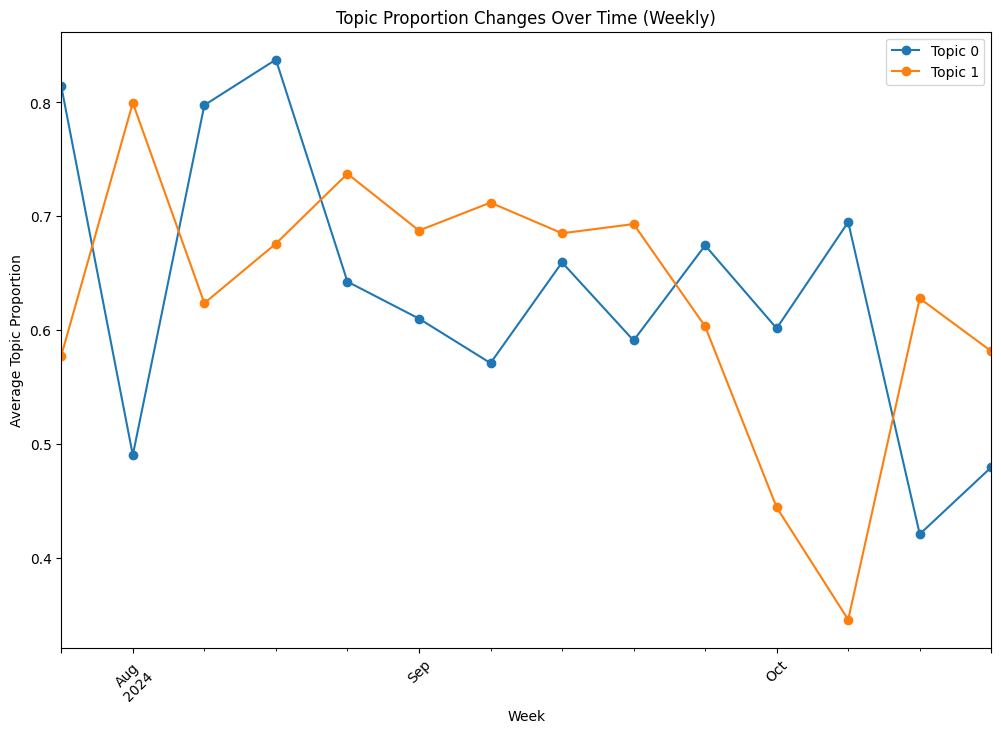
\includegraphics[width=0.8\textwidth]{topic_trends_plot.png}
        \caption{週ごとのトピック出現割合の推移(2024年7月~11月)}
        \label{fig:topic_trends}
    \end{figure}

    \chapter{分析結果に対する考察}

    本研究は、2024年10月1日のイスラエルによるレバノン侵攻がReddit上の議論やユーザーの反応に与えた影響を明らかにし、SNSが国際紛争に果たす役割を考察するものである。本章では、「はじめに」で提示した仮説と分析結果を関連付けつつ、投稿数、感情的傾向、トピックの変遷を統合的に議論する。

    \section{SNSとデジタル公共圏の形成}
    分析結果は、投稿数の急増とセンチメントスコアの変化がRedditをデジタル公共圏として機能させたことを示している。仮説1では「紛争関連サブレディットの投稿数が急増する」としたが、DID分析の結果、この仮説は支持された。

    投稿数の増加は、紛争がオンラインで公共圏を再編するプロセスを示している。この現象をハーバーマスの「公共圏」理論\citep{habermas1989structural}に照らして考えると、いくつかの特徴が明らかになる。

    まず、議論の活性化と新規ユーザーの流入が挙げられる。投稿数の急増とセンチメントスコアのポジティブな変化を関連付けると、侵攻後に新規ユーザーが流入し、議論を活性化させた可能性が高い。これにより、ネガティブなセンチメントが緩和される効果が生じたと考えられる。この現象は仮説2の修正を必要とするが、SNSが紛争の初期段階で多様な意見を取り込む力を持つことを示している。
    
    次に、情報の迅速な共有が特徴として挙げられる。紛争関連サブレディットにおける投稿数の急増は、情報が迅速に共有されると同時に、議論が特定のテーマに集中することを示している。これは、公共圏がオンラインに移行する際、特に危機的状況でその傾向が顕著になることを示唆している。
    
    ただし、SNSの公共圏としての役割には限界も存在する。アルゴリズムやエコーチェンバー現象\citep{pariser2011filter}が意見の多様性を阻害する可能性があり、これが議論の健全性にどのように影響するかはさらに検討が必要である。

    \section{感情的傾向の変化と情動の役割}
    センチメントスコアのポジティブシフトは、当初の仮説2(「ネガティブ化」)と異なる結果を示した。この結果を社会学的視点から解釈すると、いくつかの要素が浮かび上がる。
    
    まず、新規ユーザーが中立的または肯定的な意見を投稿することで、従来のネガティブな議論を緩和する役割を果たした可能性が考えられる。この現象は、デジタル空間における情動の伝播(emotional contagion)\citep{kleinberg2020emotion}が議論のトーンを変える力を持つことを示している。
    
    さらに、センチメントスコアの変化には文化的要因が関与している可能性がある。具体的には、紛争地域外のユーザーが主導する人道的支援や平和的解決を求める声が反映されていると考えられる。このような変化は、SNSが持つ国際的な性質が文化的多様性を議論に反映させる力を持つことを示している。

    これらの結果は、紛争直後のSNSが、情報共有だけでなく、情動的な安定化装置としても機能することを示唆している。

    \section{トピックの変遷と議論の多層性}
    仮説3では「議論が戦闘や人道危機から国際支援や解決策へと焦点を移す」としていたが、トピックモデリングの結果、実際には「軍事行動」や「人道危機」から「規則」や「投稿削除」へ議論が移行したことが確認された。これにより、仮説3の一部は否定されるが、議論の焦点が時間の経過とともに変化するという主張は支持された。
    
    紛争直後には「軍事行動」や「人道危機」が主要なトピックとして浮上し、議論の焦点が緊急性の高いテーマに集中していた。この急性期における議論の集中化は、SNSが紛争時において迅速な情報共有とリアルタイムの意思形成の場として機能することを示している。
    
    一方で、時間の経過とともに「規則」や「投稿削除」に関するメタ的議論が増加し、議論疲れ\citep{sunstein2001republic}や分極化が進行した可能性が示唆される。このような議論の移行は、SNSが単なる情報共有の場にとどまらず、プラットフォーム内部の規則や権力構造に対する自己批判的な議論の場としての役割を果たしていることを意味している。

    これらの結果は、SNS上の議論が現実世界の紛争と連動しつつも、その独自の動態を持つことを示している。ただし、この動態はRedditという特定のプラットフォームに依存するため、SNS全体の法則として一般化することは慎重であるべきである。

    \section{包括的結論: 仮説と結果の統合}
    本研究の分析結果は、SNSが国際紛争において多層的な役割を果たすことを示している。まず、新規ユーザーの流入が議論の内容と感情的トーンに影響を与えることで、デジタル公共圏を再編する役割を果たしていることが明らかになった。また、紛争の急性期において、情報共有と議論の集中化が進み、SNSがリアルタイムでの社会的合意形成を可能にする場として機能していることが確認された。
    
    さらに、時間の経過とともに議論疲れや分極化が進行し、SNSが単なる情報共有の場にとどまらず、自己批判的な文化を育む場としての役割を果たしていることが示唆された。これらの観点から、SNSは国際紛争の動態において多面的な影響を及ぼす重要なプラットフォームであると結論付けられる。

    ただし、これらの結論はReddit上の観察結果に基づくものであり、他のSNSや異なる文化圏では異なる動態が見られる可能性がある。本研究の結果を一般化することは慎重を要する一方で、SNSを用いた紛争対応策の設計や運営における一つの出発点として意義を持つ。

    \chapter{まとめ}
    
    \section{研究の要約}
    本研究は、2024年10月1日のイスラエルによるレバノン侵攻を契機として、Reddit上における議論の変遷を分析し、SNSが国際紛争に果たす役割を明らかにすることを目的として実施された。投稿数の変化、センチメントスコアの推移、トピックの変遷という3つの観点から多角的なデータ分析を行った結果、以下の知見が得られた。
    
    まず、投稿数の急増は、新規ユーザーの流入や紛争関連情報の共有が活発化したことを示しており、SNSがデジタル公共圏として機能する一端を明らかにした。また、センチメントスコアの分析からは、紛争直後に議論がポジティブな方向へシフトする現象が確認された。この変化は、新規ユーザーによる中立的または肯定的な意見の流入が要因であると考えられる。
    
    さらに、動的トピックモデリング(DTM)の結果、議論の焦点が「軍事行動」や「人道危機」から「規則」や「投稿削除」といったメタ的議論へと移行する傾向が観察された。これらの知見は、SNSが紛争時における情報共有や議論の進化において重要な役割を果たしていることを示している。

    これらの結果は、Redditが単なる情報共有の場にとどまらず、ユーザー間の多層的な議論やプラットフォーム内部の文化的特徴が影響を及ぼすことを示している。

    \section{研究の限界と課題}
    本研究で得られた知見にはいくつかの限界があり、それらを克服するための具体的な課題が残されている。

    \subsection{データの一般化可能性の制約}
    本研究の分析対象はRedditに限定されており、他のSNSや異なる文化圏における議論動態を考慮していない。たとえば、TwitterやFacebookといった他のプラットフォームでは、リアルタイム性やアルゴリズムの影響が議論の形成に大きな役割を果たす可能性がある。また、言語や文化的背景の異なるユーザーが議論にどのように影響を与えるかも未検討である。これを解決するためには、複数のプラットフォームを対象とし、異文化間での比較研究を進める必要がある。

    \subsection{感情分析の精度向上}
    感情分析に使用したVADERは、SNSデータに特化して設計されている一方で、皮肉や隠喩、文化的文脈に依存する表現を十分に捉えられない可能性がある。この限界を克服するため、深層学習を用いた感情分析モデルの導入や、人間の評価によるデータの補正を組み合わせることが有効である。また、言語的多様性を考慮し、多言語対応の感情分析モデルを採用することで、分析の信頼性をさらに高めることが期待される。

    \subsection{長期的な議論の動態の追跡}
    本研究の分析期間は約3か月間であり、紛争の初期段階に焦点を当てている。これにより、議論が時間の経過とともにどのように発展し、沈静化するかについての包括的な理解には至っていない。今後の研究では、長期間のデータを収集し、議論の成長、疲弊、そして再構築のプロセスを時系列的に分析する必要がある。

    \subsection{特定の事例に限定された知見の課題}
    本研究は、「イスラエルによるレバノン侵攻」という特定の紛争事例を対象としており、SNSと紛争の関係性に関する一般法則を示すまでには至っていない。このような単一事例の分析では、結果が特定の文化的背景や地域的特性に依存している可能性がある。そのため、一般化可能な知見を得るためには、異なる地域や紛争の種類にまたがる比較研究を行う必要がある。たとえば、ウクライナ紛争や南シナ海問題など、異なる地政学的文脈におけるSNSの役割を分析することで、SNSが国際紛争全般において果たす役割をより包括的に理解できる可能性がある。

    \section{研究結果の具体的な意義}
    本研究で得られた知見は、SNSの活用や規制に関して具体的な指針を提供するものである。まず、紛争急性期における投稿数の急増とトピック集中化の観察結果は、SNSが迅速な情報共有とリアルタイムの世論形成を可能にする重要なツールであることを示している。この点で政策立案者にとっては、SNSを活用して国際社会の関心を喚起し、被害状況の可視化を図ることで、国際的な支援や介入を効果的に促進する可能性がある。
    
    また、本研究は、新規ユーザーの流入が議論のトーンやトピックに与える影響を示しており、これを活用して紛争地域外の声を集める仕組みを設計することで、議論の多様化と偏りの是正が期待できる。この点でプラットフォーム運営者にとっては、議論が閉鎖的なエコーチェンバーに陥らないよう、アルゴリズムの調整が重要であることが示唆される。
    
    さらに、後期におけるメタ議論の増加と議論疲れの進行を踏まえ、プラットフォーム運営者は議論の健全性を維持するためのモデレーション手法を見直す必要がある。たとえば、長期間続く議論には、新たな視点を提供するためのキュレーション機能や、議論の焦点を再設定する仕組みを導入することが効果的であると考えられる。
    
    最後に、本研究の結果は、SNSがデジタル公共圏として機能する可能性を示唆している。一方で、公共圏の形成には、特定の視点が過剰に強調されないような設計が求められる。この点でプラットフォーム運営者は、アルゴリズムの透明性を向上させ、多様な意見が均等に可視化される仕組みを開発することが求められる。
    
    \section{結論}
    本研究は、2024年のイスラエルによるレバノン侵攻を題材に、Redditにおける投稿データを分析することで、SNSが国際紛争において果たす役割とその限界を明らかにした。本研究の成果は、デジタル時代における公共圏の新たな形態を理解するための基盤を提供するとともに、SNS運営者や政策立案者がより健全で多様な議論環境を構築するための実践的な示唆を与えるものである。

    %=====================================================================================

    \addcontentsline{toc}{chapter}{参考文献} %章立てせずに目次に追加するおまじない
    \renewcommand{\bibname}{参考文献} %これがないと,タイトルが「関連図書」になってしまう
    \bibliographystyle{chicago} %本文に\citep{}を入れることで,参考文献表示
    \bibliography{main.bib} %bibtexファイルの読み込み
\end{document}
